\chapter{Stacionární procesy ve frekvenční doméně}

\section{Úvod}

V předchozím textu jsme se zabývali několika typy stacionárních procesů, jejichž vývoj v čase jsme analyzovali pomocí autokovarianční popř. autokorelační funkce. V následujícím textu se budeme zabývat frekvenčními vlastnosti vybraných stacionárních procesů - namísto časové domény budeme stacionární procesy analyzovat ve frekvenční doméně. Roli autokovarianční / autokorelační funkce převezme tzv. spektrální funkce hustoty.

Analýza procesů ve frekvenční doméně je běžně používána v elektroinženýrství, geofyzice nebo meteorologii. V následujícím textu se omezíme na reálné procesy. Existují také komplexní procesy, nicméně většina praktických problémů má charakter právě reálných procesů.

\section{Spektrální distribuční funkce}

V následujícím textu si představíme spektrální distribuční funkci. Přístup, který zde aplikujeme, je heuristický, nicméně věříme, že čtenáře do problematiky uvede lépe než matematicky rigorózní výklad.

Předpokládejme, že časová řada obsahuje periodickou sinusoidní komponentu se známou vlnovou délkou. Tuto řadu můžeme vyjádřit je formě
\begin{equation}
X_t = R \cos(\omega t + \theta) + Z_t,
\end{equation}
kde $\omega$ představuje frekvenci, $R$ amplitudu, $\theta$ fázi a $Z_t$ obecnou stacionární časovou řadu. Úhel $(\omega t + \theta)$ je obvykle měřen v radiánech. Protože parametr $\omega$ vyjadřuje počet radiánu za jednotku času, nazýváme jej někdy také úhlovou rychlostí. Někteří autoři pojmem frekvence neoznačují $\omega$ nýbrž $f = \frac{\omega}{2 \pi}$, což představuje počet cyklů za jednotku času. Jedna perioda sinusoidního cyklu, označovaná též jako vlnová délka, je tak $1/f$ resp. $2\pi/ \omega$. Příklad sinusoidní funkce s vlnovou délkou 6 je uveden na obrázku (6.1).

\begin{figure}[htp]
\centering
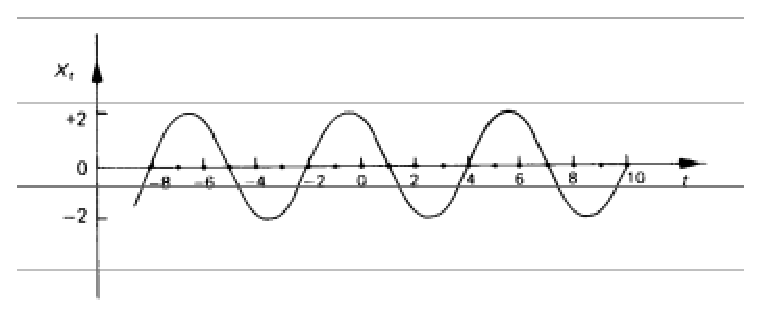
\includegraphics[scale = 0.75]{pictures/figure_6_1.eps}
\caption{Graf $R \cos(\omega t + \theta)$ s $R=2$, $\omega = \pi / 3$ a $\theta = \pi / 6$.}
\label{figure_6_1}
\end{figure}

V praxi může být variace časové řady způsobena variací na několika různých frekvencích. Proto je běžné (6.1) zobecnit do tvaru
\begin{equation}
X_t = \sum_{j=1}^k R_j \cos(\omega_j t + \theta_j) + Z_t,
\end{equation}
kde $R_j$ je amplituda ve frekvenci $\omega_j$.

Je zřejmé, že modely (6.1) a (6.2) nejsou stacionární, pokud $R$, $\theta$, $\{R_j\}$ a $\{\theta_j\}$ jsou konstanty, protože se $E(X_t)$ mění v čase. Abychom byli schopni aplikovat teorii stacionárních řad na modely typu (6.2), obvykle předpokládáme, že $\{R_j\}$ jsou nekorelované náhodné veličiny s nulovou střední hodnotou nebo že $\{\theta_j\}$ jsou náhodné veličiny se stejnoměrným rozdělením na intervalu $(0, 2 \pi)$, které jsou zafixované pro jednu konkrétní realizaci procesu. Pomocí tohoto ``matematického triku'' jsme schopni na časovou řadu obsahující jednu nebo vícero deterministických sinusoidních komponent nahlížet jako na stacionární.

Protože $\cos(\omega t + \theta) = \cos \omega t \cos \theta - \sin \omega t \sin \theta$, lze model (6.2) také vyjádřit ve tvaru
\begin{equation}
X_t = \sum_{j=1}^k (a_j \cos \omega_j t + b_j \sin \omega_j t) + Z_t,
\end{equation}
kde $a_j = R_j \cos \theta_j$ a $b_j = - R_j \sin \theta_j$.

Přirozenou otázkou je, proč by měl model (6.2) resp. (6.3) zahrnovat pouze konečný počet frekvencí. Wiener dokázal, že pro $k \rightarrow \infty$ lze libovolný diskrétní stacionární proces měřený v jednotkových intervalech vyjádřit ve formě
\begin{equation}
X_t = \int_0^{\pi} \cos \omega t du(\omega) + \int_0^{\pi} \sin \omega t dv(\omega),
\end{equation}
kde $u(\omega)$ a $v(\omega)$ jsou nekorelované spojité procesy s ortogonálními přírůstky, které jsou definované pro všechna $\omega$ v intervalu $(0, \pi)$. Rovnice (6.4) se nazývá spektrální reprezentací procesu a obsahuje stochastické integrály, které jsou poměrně komplikované a přesahují záběr této knihy. Pro intuitivní pochopení problému je vhodnější ignorovat problematiku stochastických integrálů a jednoduše nahlížet na $X_t$ jako na lineární kombinaci ortogonálních sinusoidních přírůstků.

Čtenář se může pozastavit nad tím, proč horní meze integrálu v (6.4) jsou $\pi$ spíše než $\infty$. Pro kontinuální procesy by horní meze byly opravdu rovny $\infty$, ale pro diskrétní procesy měřené v jednotkových časových intervalech můžeme bez ztráty zobecnění omezit $\omega$ na interval $(0, \pi)$, protože
\begin{equation}
\cos[(\omega + k \pi)t] = 
\begin{cases}
\cos \omega t \quad \textit{$k$, $t$ celá čísla; $k$ je sudé}\\
\cos(\pi - \omega)t \quad \textit{$k$, $t$ celá čísla; $k$ je liché}\\
\end{cases}
\end{equation}
a tak nejsme schopni odlišit variace na frekvenci vyšší než $\pi$ od variace na odpovídající frekvenci z intervalu $(0, \pi)$. Frekvence $\omega = \pi$ se nazývá Nyquistova frekvence a podrobněji se o ní zmíníme v následující kapitole. Pro diskrétní procesy měřené v konstantních intervalech $\delta t$ je Nyquistova frekvence rovna $\pi / \Delta t$.

Hlavním důvodem uvedení spektrální reprezentace ve formě (6.4) je ukázat, že libovolná frekvence v intervalu $(0, \pi)$ může přispívat do variace procesu. Nicméně procesy $u(\omega)$ a $v(\omega)$ v (6.4) mají jen omezený praktický význam. Namísto nich představíme funkci $F(\omega)$, kterou nazýváme spektrální distribuční funkcí a která vychází z tzv. Wiener-Khintchinova teorému. Tento teorém říká, že pro libovolný stacionární stochastický proces s autokovarianční funkcí $\gamma(k)$ existuje monotónně rostoucí funkce $F(\omega)$ taková, že
\begin{equation}
\gamma(k) = \int_0^{\pi} \cos \omega k ~ d F(\omega).
\end{equation}
Tato rovnice se nazývá spektrální reprezentací autokovarianční funkce a obsahuje tzv. Stieltjesův integrál. Funkce $F(\omega)$ má přímou fyzikální interpretaci - jedná se ``příspěvek'' frekvencí z intervalu $(0, \pi)$ do variace zkoumané časové řady. Protože záporné frekvence do variace nepřispívají, platí
\begin{equation}
F(\omega) = 0 \quad \omega < 0.
\end{equation}
Pro diskrétní procesy měřené v jednotkových časových intervalech je nejvyšší možná frekvence rovna $\pi$, a proto
\begin{equation}
F(\pi) = Var(X_t) = \sigma_X^2,
\end{equation} 
což lze odvodit z (6.6) pro $k = 0$, kde
\begin{equation}
\gamma(0) = \sigma_X^2 = \int_0^{\pi} dF(\omega) = F(\pi).
\end{equation}
Mezi $\omega = 0$ a $\omega = \pi$ je $F(\omega)$ monotónně rostoucí.

Jestliže proces obsahuje deterministickou sinusoidní komponentu na frekvenci $\omega_0$, řekněme $R ~ \cos (\omega_0 t + \theta)$, kde $R$ je konstanta a $\theta$ je z intervalu $(0, 2 \pi)$, pak bude $F(\omega)$ vykazovat v $\omega_0$ ``schod'' ve výši $E[R^2 \cos^2(\omega_t + \theta)] = \frac{1}{2}R^2$.

Protože je funkce $F(\omega)$ monotonní, může být rozdělena na dvě funkce $F_1(\omega)$ a $F_2(\omega)$ tak, že
\begin{equation}
F(\omega) = F_1(\omega) + F_2(\omega),
\end{equation}
kde $F_1(\omega)$ je neklesající spojitá funkce a $F_2(\omega)$ je neklesající schodová funkce. Dekompozice obvykle odpovídá Woldově dekompozici, kde $F_1(\omega)$ představuje stochastickou a $F_2(\omega)$ deterministickou část procesu. V následujícím textu se budeme převážně zabývat stochastickou částí procesu, a proto $F_2(\omega) \equiv 0$, což znamená, že $F(\omega)$ je spojitá funkce na intervalu $(0, \pi)$.

Někteří autoři používají normalizovanou verzi funkce $F(\omega)$ definovanou jako
\begin{equation}
F^*(\omega) = \frac{F(\omega)}{\sigma_X^2}.
\end{equation}
Funkci $F^*(\omega)$ tak lze interpretovat jako poměrnou část celkového rozptylu, která je dána frekvencemi z intervalu $(0, \omega)$. Protože $F^*(\pi) = 1$ a $F^*(\omega)$ je monotónně rostoucí, má $F^*(\omega)$ podobné vlastnosti jako kumulativní distribuční funkce.

\section{Spektrální funkce hustoty}

V případě stochastického diskrétního stacionárního procesu je spektrální funkce hustoty spojitou monotónní funkcí definovanou na intervalu $(0, \pi)$, která je definována jako
\begin{equation}
f(\omega) = \frac{dF(\omega)}{d \omega}.
\end{equation}
Rovnici (6.6) tak lze vyjádřit pomocí Riemanova integrálu jako
\begin{equation}
\gamma(k) = \int_0^{\pi} \cos \omega k f(\omega) d\omega.
\end{equation}
Pro $k = 0$ získáváme
\begin{equation}
\gamma(0) = \sigma_X^2 = \int_0^{\pi} f(\omega) d \omega = F(\pi).
\end{equation}
Fyzikální význam spektrální funkce hustoty je ten, že $f(\omega) d \omega$ představuje ``příspěvek'' komponent s frekvencí z intervalu $(\omega, \omega + d \omega)$ do celkového rozptylu procesu. Rovnice (6.14) nám pak říká, že plocha pod křivkou $f(\omega)$ je rovna rozptylu procesu. Lokální maxima této funkce navíc indikuje ty frekvence, které to celkového rozptylu přispívají nejvíce.

\begin{figure}[htp]
\centering
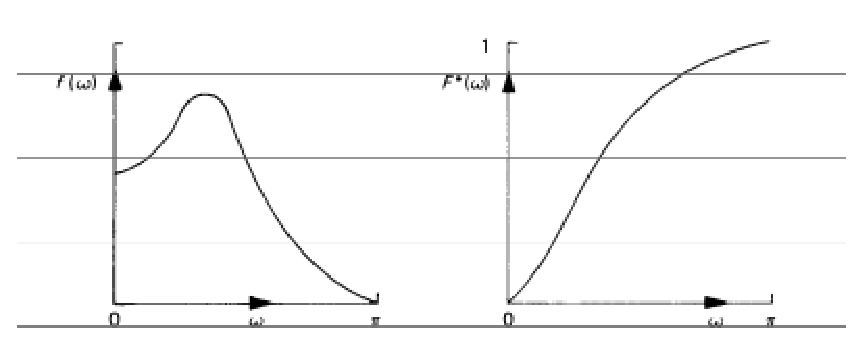
\includegraphics[scale = 0.75]{pictures/figure_6_2.eps}
\caption{Příklad spektrální funkce hustoty $f(\omega)$ a odpovídající spektrální kumulativní distribuční funkce $F^*(\omega)$}
\label{figure_6_2}
\end{figure}

Je důležité si uvědomit, že autokovarianční funkce a spektrální funkce hustoty představují dva ekvivalentní popisy stochastického stacionárního procesu. Obě funkce obsahují tutéž informaci, kterou však ``předávají'' různým způsobem. V některých případech je vhodnější využít autokovarianční funkci založenou na časovém přístupu, jindy pak spektrální funkci hustoty založenou na frekvenčním přístupu.

Rovnice (6.13) vyjadřuje $\gamma(k)$ s pomocí $f(\omega)$. Inverzní vztah
\begin{equation}
f(\omega) = \frac{1}{\pi} \sum_{k = -\infty}^{\infty} \gamma(k)e^{-i \omega k}
\end{equation}
lze odvodit pomocí Fourierovy transformace. Protože je $\gamma(k)$ sudou funkcí, je (6.15) často vyjádřena v ekvivalentní formě
\begin{equation}
f(\omega) = \frac{1}{\pi}\Big[\gamma(0) + 2 \sum_{k = 1}^{\infty} \gamma(k) \cos \omega k \Big].
\end{equation}
Pokud bychom (6.16) aplikovali na proces obsahující deterministickou komponentu na frekvenci $\omega_0$, pak by $\sum \gamma(k) \cos \omega_0 k$ nekonvergovalo, protože by $F(\omega)$ nebylo diferencovatelné v $\omega_0$, a proto by $f(\omega_0)$ nebylo definované.

V literatuře je možné se setkat také jinými definicemi spektrální funkce hustoty. Asi nejznámější přístup definuje spektrální funkci hustoty na intervalu $(-\pi, \pi)$ jako
\begin{equation}
f(\omega) = \frac{1}{2 \pi} \sum_{k = -\infty}^{\infty} \gamma(k) e^{-i \omega k}
\end{equation}
s inverzním vztahem ve tvaru
\begin{equation}
\gamma(k) = \int_{-\pi}^{\pi} e^{i \omega k} f(\omega) d \omega.
\end{equation}

Někdy je užitečné použít normalizovanou formu spektrální funkce hustoty
\begin{equation}
f^*(\omega) = \frac{f(\omega)}{\sigma_X^2} = \frac{dF^*(\omega)}{d \omega}.
\end{equation}
Lze dokázat, že $f^*(\omega)$ je Fourierovou transformací autokorelační funkce, konkrétně pak
\begin{equation}
f^*(\omega) = \frac{1}{\pi}\Big[1 + 2 \sum_{k = 1}^{\infty} \rho(k) \cos \omega k \Big],
\end{equation}
a že $f^*(\omega)$ představuje poměrnou část rozptylu z frekvencí na intervalu $(\omega, \omega + d\omega)$.

\section{Spektrální funkce hustoty spojitého procesu}

V případě spojitého deterministického stacionárního procesu je autokovarianční funkce $\gamma(\tau)$ definována pro všechna $\tau$ a spektrální funkce hustoty $f(\omega)$ pak pro všechna kladná $\omega$. Spojitost mezi oběma funkcemi je podobná jako v případě diskrétního procesu s tou výjimkou, že neexistují dolní a horní integrální mez. Konkrétně platí
\begin{equation}
f(\omega) = \frac{1}{\pi} \int_{-\infty}^{\infty} \gamma(\tau) e^{-i \omega \tau} d \tau = \frac{2}{\pi} \int_0^{\infty} \gamma(\tau) \cos \omega \tau d \tau
\end{equation}
pro $0 < \omega < \infty$ a
\begin{equation}
\gamma(\tau) = \int_0^{\infty} f(\omega) \cos \omega \tau d \omega.
\end{equation}

\section{Spektrální funkce vybraných procesů}

\subsection{Čistě náhodný proces}

Čistě náhodný diskrétní proces $\{Z_t\}$ je definován v kapitole 3.4.1. Jestliže $Var(Z_t) = \sigma_Z^2$, pak je autokovarianční funkce dána
\begin{equation}
\gamma(k) =
\begin{cases}
\sigma^2_Z \quad k = 0\\
0 \quad \textit{v ostatních případech}
\end{cases}
\end{equation}
a s pomocí (6.16) lze odvodit spektrální funkci hustoty
\begin{equation}
f(\omega) = \frac{\sigma^2_Z}{\pi}.
\end{equation}
To znamená, že spektrální funkce je v intervalu $(0, \pi)$ konstantní.

V předchozím textu jsme zmiňovali, že fyzická realizace bílého šumu je nemožná. Nicméně proces, který lze považovat za praktickou aproximaci spojitého bílého šumu, je definován spektrální funkcí hustoty ``dostatečně'' konstantní v relevantním intervalu frekvencí.

\subsubsection{MA(1) proces}

MA(1) proces je definován jako
\begin{equation}
X_t = Z_t + \beta Z_{t-1}
\end{equation}
a má autokovarianční funkci ve tvaru
\begin{equation}
\rho(k) = 
\begin{cases}
1 \quad k = 0\\
\frac{\beta}{1 + \beta^2} \quad k \pm 1\\
0 \quad \textit{v ostatních případech}.
\end{cases}
\end{equation}
S využitím (6.20) lze odvodit normalizovanou spektrální funkci hustoty ve tvaru
\begin{equation}
f^*(w) = \frac{1}{\pi}\Big[1 + \frac{2 \beta \cos \omega}{1 + \beta^2}\Big]
\end{equation}
pro $0 < \omega < \pi$. Spektrální funkce hustoty pak má tvar
\begin{equation}
f(\omega) = \sigma_X^2 f^* (\omega),
\end{equation}
kde $\sigma_X^2 = (1 + \beta^2) \sigma_Z^2$.

Tvar spektrální funkce hustoty se odvíjí od hodnoty parametru $\beta$. Pro $\beta > 0$ je ``hustota'' koncentrována v nižších frekvencích; pro $\beta < 0$ je tomu naopak. Situaci ilustruje obrázek (6.3).

\begin{figure}[htp]
\centering
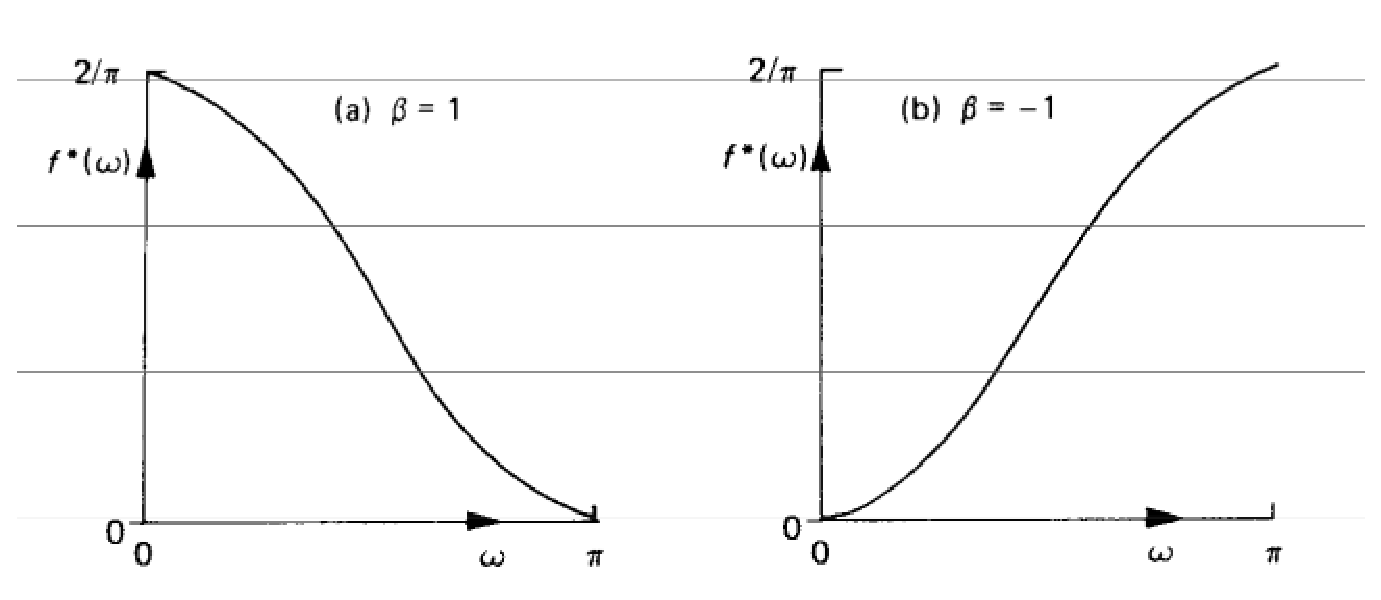
\includegraphics[scale = 0.50]{pictures/figure_6_3.eps}
\caption{Příklady spektrální funkce hustoty MA(1) procesu pro $\beta=1$ a $\beta=-1$.}
\label{figure_6_3}
\end{figure}

\subsection{AR(1) proces}

AR(1) proces je definován jako
\begin{equation}
X_t = \alpha X_{t - 1} + Z_t
\end{equation}
a jeho autokovarianční funkce má tvar
\begin{equation}
\gamma(k) = \sigma_Z^2 \alpha^{|k|} \quad k = 0, \pm 1, \pm 2, ...
\end{equation}
S využitím (6.15) lze odvodit spektrální funkci hustoty
\begin{align}
f(\omega) = \frac{\sigma_X^2}{\pi} \Big(1 + \sum_{k = 1}^{\infty} \alpha^k e^{-ik \omega} + \sum_{k = 1}^{\omega} \alpha^k e^{ik\omega}\Big)\\
= \frac{\sigma_X^2}{\pi} \Big(1 + \frac{\alpha e^{-i \omega}}{1 - \alpha e^{-i \omega}} + \frac{\alpha e^{i \omega}}{1 - \alpha e^{i \omega}} \Big),
\end{align}
což lze s pomocí $e^{inx} = \cos nx + i \sin nx$ a $\sigma_Z^2 = \sigma_X^2(1 - \alpha^2)$ dále upravit do tvaru
\begin{equation}
f(\omega) = \frac{\sigma_X^2(1 - \alpha^2)}{\pi(1 - 2\alpha \cos \omega + \alpha^2)} = \frac{\sigma_Z^2}{\pi(1 - 2 \alpha \cos \omega + \alpha^2)}.
\end{equation}

Tvar spektrální funkce AR(1) procesu závisí na hodnotě $\alpha$. Pro $\alpha > 0$ je ``hustota'' koncentrovaná v nižších frekvencích; pro $\alpha > 0$ je tomu naopak. Situaci ilustruje obrázek (6.4).

\begin{figure}[htp]
\centering
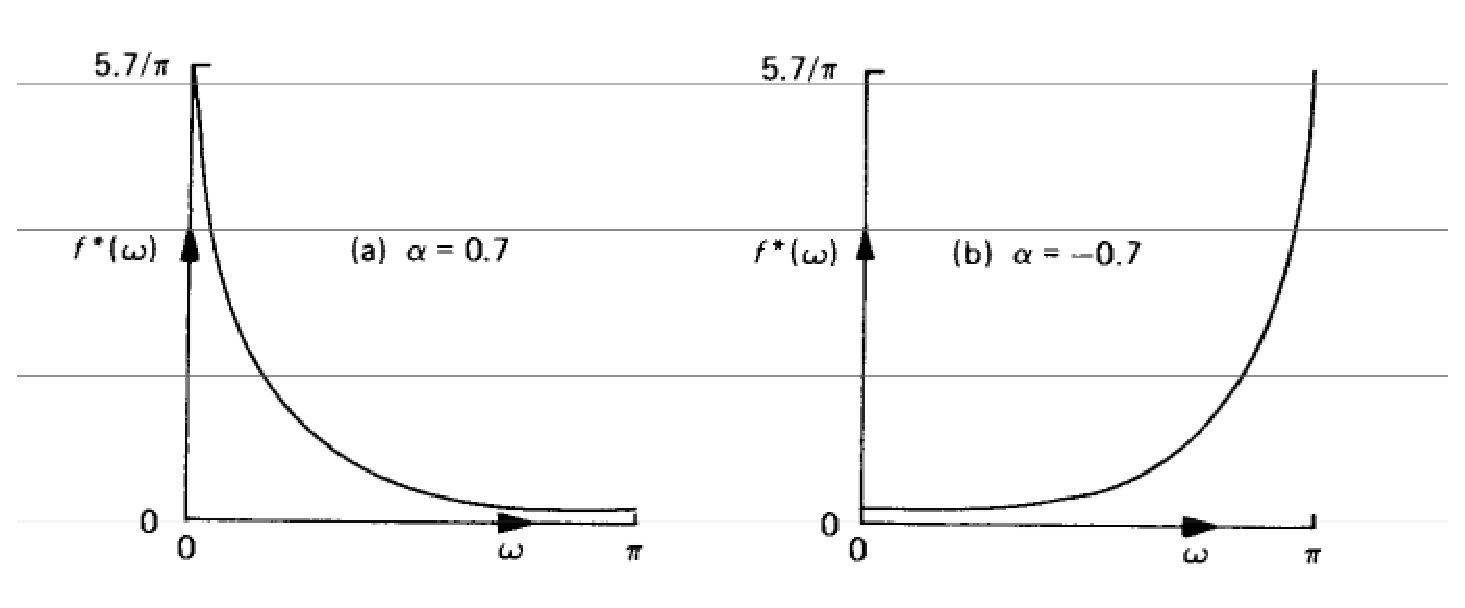
\includegraphics[scale = 0.50]{pictures/figure_6_4.eps}
\caption{Příklady spektrální funkce hustoty AR(1) procesu pro $\alpha=0.7$ a $\alpha=-0.7$.}
\label{figure_6_4}
\end{figure}

Interpretace obrázku (6.4) je intuitivní. Pokud je např. $\alpha$ záporné, pak je z (6.29) zřejmé, že hodnota $X_t$ bude mít tendenci oscilovat, přičemž rychlá oscilace odpovídá vysokému rozptylu ve vysokých frekvencích.

\subsection{AR procesy vyššího řádu}

Spektrální funkce hustoty AR(2) procesu s parametry $\alpha_1$ a $\alpha_2$ je dána
\begin{equation}
f(\omega) = \frac{\sigma_Z^2}{\pi[1 + \alpha_1^2 + \alpha_2^2 - 2 \alpha_1(1 - \alpha_2) \cos \omega - 2 \alpha_2 \cos 2 \omega]}
\end{equation}
pro $0 < \omega < \pi$. Tvar spektrální funkce závisí na parametrech $\alpha_1$ a $\alpha2$. V závislosti na jejich hodnotách je možné získat funkci, která je koncentrovaná v nižších popř. vyšších frekvencích nebo která má minimum popř. maximum v intervalu $(0, \pi)$.

V případě AR procesů vyššího řádu můžeme získat spektrální funkci hustoty, která má několik lokálních minim či maxim.

\subsection{Deterministický sinusoidní proces}

Uvažujme proces
\begin{equation}
X_t = \cos(\omega_0 t + \theta),
\end{equation}
kde $\omega_0$ je konstanta z intervalu $(0, \pi)$ a $\theta$ je náhodná veličina, která je stejnoměrně rozdělená nad intervalem $(0, 2 \pi)$. Jak bylo vysvětleno v kapitole 3.5, pokud je $\theta$ fixní pro jednu realizaci procesu, představuje (6.35) čistě deterministický proces. Jeho autokovarianční funkce je dána rovnicí
\begin{equation}
\gamma(k) = \frac{1}{2}\cos \omega_0 k.
\end{equation}
Autokorelační funkce tohoto procesu neklesá k nule s rostoucím $k$, což je vlastnost většiny deterministických procesů.

Z (6.35) je patrné, že ``hustota'' procesu je koncentrována ve frekvenci $\omega_0$. Protože $Var(X_t) = E(X_t^2) = \frac{1}{2}$, má spektrální distribuční funkce podobu
\begin{equation}
F(\omega) =
\begin{cases}
0 \quad \omega < \omega_0\\
\frac{1}{2} \quad \omega \ge \omega_0.
\end{cases}
\end{equation}
Protože se jedná o schodovou funkci, nemá derivaci v bodě $\omega_0$, a proto není spektrální funkce hustoty v tomto bodě definována. S pomocí rovnice (6.16) a Fourierovy transformace autokovarianční funkce jsme však schopni dokázat, že
\begin{equation}
f(\omega) = 0 \quad \omega \ne \omega_0,
\end{equation}
a že $\sum \gamma(k) \cos \omega k$ v $\omega = \omega_0$ nekonverguje.

\subsection{Mix deterministického a stochastického procesu}

Uvažujme proces
\begin{equation}
X_t = \cos(\omega_0 t + \theta) + Z_t,
\end{equation}
který obsahuje deterministickou a stochastickou složku, kde $\omega_0$ a $\theta$ jsou definovány stejně jako v předchozím případě a $\{Z_t\}$ je čistě náhodný proces s nulovou střední hodnotou a rozptylem $\sigma_Z^2$. Autokovarianční funkce tohoto procesu má podobu
\begin{equation}
\gamma(k) =
\begin{cases}
\frac{1}{2} + \sigma_Z^2 \quad k = 0\\
\frac{1}{2} \cos \omega_0 \quad k = \pm 1, \pm 2, ...
\end{cases}
\end{equation}
Všimněme si, že $\gamma(k)$ neklesá s rostoucím $k$ k nule, protože $X_t$ obsahuje deterministickou komponentu.

Spektrální distribuční funkci můžeme odvodit s pomocí (6.10), kde deterministická složka $\cos (\omega_0 t + \theta)$ má distribuční funkci
\begin{equation}
F_1(\omega) =
\begin{cases}
0 \quad \omega < \omega_0\\
\frac{1}{2} \quad \omega \ge \omega_0
\end{cases}
\end{equation}
a stochastická složka $Z_t$ pak
\begin{equation}
F_2(\omega) = \frac{\sigma_Z^2 \omega}{\pi} \quad 0 < \omega < \pi,
\end{equation}
což lze odvodit integrací (6.24). Výsledná spektrální distribuční funkce tak má podobu
\begin{equation}
F(\omega) =
\begin{cases}
\frac{\sigma_Z^2 \omega}{\pi} \quad 0 < \omega < \omega_0\\
\frac{1}{2} + \frac{\sigma_Z^2 \omega}{\pi} \quad \omega_0 \ge \omega < \pi.
\end{cases}
\end{equation}
Stejně jako v předchozím případě není tato funkce definována v bodě $\omega = \omega_0$.
